\section{Conclusion}
\subsection{}
\begin{frame}
 \frametitle{Conclusion}
 Pour beaucoup d'applications , le temps de vie de la batterie est satisfaisant.\\
 (Pour 40 octets toutes les 10 minutes, impact sur la batterie de 10,84\%.
 %De plus, en utilisant leur design, l'implémentation de services web sur un capteur est peu gourmand en calculs et mémoires.
 %Par exemple, le parser XML est simplifié car le capteur ne répond qu'au message spécifié dans sa déscription WSDL.
\end{frame}

\begin{frame}
 \frametitle{Problèmes}
 \begin{itemize}
  \item \textbf{Sleep mode}: Comment s'assurer que tous les échanges de messages dans la couche réseaux soient designés pour le sleep mode ?
  \item \textbf{Multi-hop connection}: Et si le message doit passer par plusieurs capteurs pour atteindre le controleur ?\\
  Alors chaque capteur intermédiaire doit envoyer des messages wake-up, maintenir une liste d'adresse MAC...Tout cela va créer de l'overhead
  \item \textbf{Sécurité}: Comment assurer la sécurité entre un capteur et un controleur ?\\
  %Il vaut mieux éviter de crypter un paquet 6lowpan pour qu'il puisse être converti en IPv6 sans dévoir décrypter.\\
  CC2420 crypte et décrypte en hardware en définissant quelle partie il faut crypter.
  Ainsi la conversion 6lowpan à IPv6 se fait sans devoir décrypter le message.\\
  Si la clé est échangée en ligne, la proximité des deux appareils réduit les risques d'écoutes indiscrètes.
  %Ce qui n'est pas très convainquant en terme de Sécurité
  Ou alors on transmet manuellement la clé.
 \end{itemize}
\end{frame}

\begin{frame}
 \frametitle{Résultats du prototype}
 %Grâce à un algorithme qui baisse la température du chauffage lorsque la maison est innocupée, ils ont pu économiser 7,2\% d'énergie de chauffage.\\
 Économie totale d'énergie par jour:
 \begin{figure}
  \centering
  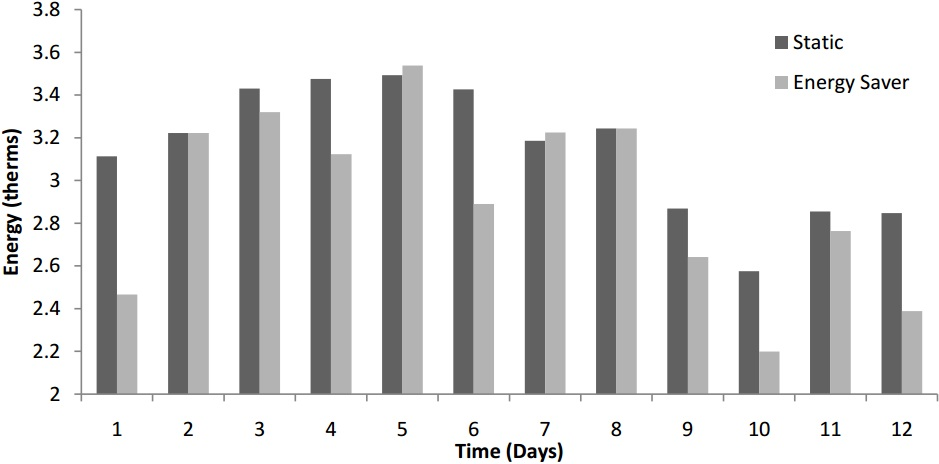
\includegraphics[scale=0.38]{figures/energysaver.jpg}
  \caption{Économie d'énergie totale}
 \end{figure} 
\end{frame}